\documentclass{article}
\usepackage[english]{babel}
\usepackage[utf8]{inputenc}
\usepackage{amsmath}
\usepackage{amsfonts}
\usepackage{amsthm}
\usepackage{hyperref} % For hyperlinks
\usepackage{graphicx} % To use figures
\usepackage{biblatex} % For citations
\addbibresource{refs.bib}

% Add in the definition environment
\theoremstyle{definition}
\newtheorem{definition}{Definition}[section]

% Add useful operators and commands

\DeclareMathOperator{\Tr}{Tr}
\DeclareMathOperator{\Diag}{Diag}
\newcommand{\norm}[1]{\left\lVert#1\right\rVert}

\hypersetup{
    colorlinks=true,
    linkcolor=blue,
    filecolor=magenta,      
    % urlcolor=blue,
    pdftitle={Overleaf Example},
    pdfpagemode=FullScreen,
    }

\title{Senior Thesis}
\author{Abhi Uppal}
\date{December 2021}

\begin{document}

\maketitle

\newpage

\section{Introduction and Literature Review}
\label{sec:intro}

Graph theory is a particularly flexible mathematical language for modeling the relationship between different entities. While it is a vague description, it draws its power from this -- providing a framework for analyzing problems ranging all the way from social network analysis \cite{socialNetworkAnalysis} to creating a model of natural language \cite{speer2018conceptnet}. 

Once one has a graph structure, one can apply a plethora of algorithms to understand the statistics of the graph -- which entities are the big players, how strongly connected are each of the entities, how many hops would it take to get from one end of the graph to the other, and many more. 

In this section, I provide a high-level overview of graphs, as well as some rigorous mathematical definitions of graphs and some node features. I then discuss some of the applications of graph theory before pivoting into a discussion of the problem at hand in this project: how to optimally infer edge weights for a graph whose nodes represent different time series, with the goal of modeling the relationships between the time series by considering how they evolve together in time. Within this discussion, I cover the data I will use for the two main case studies for applications of this model.

After this section, I present the novel methodology -- a nonlinear Gaussian noise model that learns through stochastic gradient descent a graph and a Gaussian covariance matrix based on how different series move together in time. Following the methodology, I present the results of the algorithm and conclusions. Past the conclusions section is the Appendix, where all of the mathematical work is done. In the ppendix, I assume some familiarity with matrix calculus. I invite the reader to consult the Matrix Cookbook \cite{matrixCookbook} as a reference.

The interested reader may find the code used for this paper available at \href{https://github.com/AbhiUppal/seniorthesis}{\texttt{https://github.com/AbhiUppal/seniorthesis}}.

\subsection{A High-Level Overview of Graphs}
\label{sec:graphOverview}

A modern understanding of the world, whether quantitative or qualitative, seldom permits the ability to understand phenomena in isolation. One of the most prominent ways we see this is in the humanities, where scholars will attempt to understand issues as the complex combination of multiple causes. A popular example is Mark Juergensmeyer's \textit{Terror in the Mind of God} \cite{terrorInTheMindOfGod}, where he attempts to understand global violence and terrorism through the intersection of politics and religion -- two somewhat disparate topics with a sizable overlap. Looking at each factor alone, while informative, cannot provide the full picture. Rather, it is also the \textit{relationship between} factors that can often provide informative signals towards the truth.

So, how does this method of inquiry manifest itself in quantitative terms? The idea is rooted in an application of \textit{graph theory}, one of the most flexible fields of mathematics. We represent the objects we wish to understand as agents, or nodes, in a network (henceforth referred to as a \textit{graph}). These nodes are connected to each other via edges that quantify and/or categorize the relationship between them. For example, in a graph describing things we might see in a suburban neighborhood, we might have a node for ``person" and ``car". How might we write the relationship between them? We might write,

\begin{center}
    person $\xrightarrow{\text{DRIVE}}$ car,
\end{center}

where ``DRIVE" is a type of edge connecting the ``person" and ``car" nodes, denoting that ``DRIVE" is an action that ``person" can take with ``car". Similarly, we might have another edge

\begin{center}
    person $\xrightarrow{\text{FIX}}$ car,
\end{center}

denoting that ``person" can also fix the object represented by ``car". As a final example, we might have

\begin{center}
    car $\xrightarrow{\text{PARK\_IN}}$ driveway,
\end{center}

denoting that ``PARK\_IN" is also an action that the object represented by ``car" can take with the object represented by ``driveway". Following this process to construct more nodes and edges, we may end up with a graph that describes pretty well how the components of a suburban neighborhood might act with each other, giving us a clear picture of how they might operate on a day-to-day basis.

\begin{figure}[hbt!]
\vspace{-0.125in}
\par
\begin{center}
\caption{Simple Heterograph Toy Example}
\vspace{0.1in}
\label{fig:simpleHetGraph}
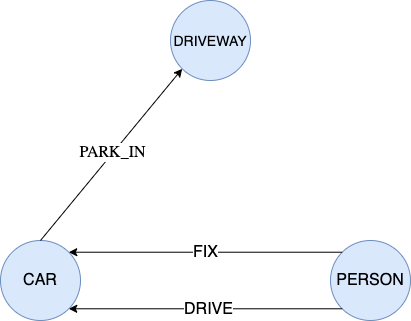
\includegraphics[scale=0.4]{Figures/SimpleHetGraph.png}
\end{center}
\par
\vspace{-0.25in}
\medskip
\end{figure}

Obviously, in this toy example, we understand what each of these nodes and edges represent. It may seem pointless to go through this exercise, but the importance lies in the abstraction. What if we didn't aptly name the nodes, but created a set of nodes $V = \{1, 2, 3, \dots, n\}$, but we kept the same relationships? So, 1 $\xrightarrow{\text{DRIVE}}$ 2, 1 $\xrightarrow{\text{FIX}}$ 2, and 2 $\xrightarrow{\text{PARK\_IN}}$ 3. From a mathematical perspective, assigning the word ``car" is just as arbitrary as assigning the number $1$ to a node. In a similar sense, the edge names ``DRIVE", ``FIX", ``PARK\_IN" are also completely arbitrary. They make sense to us, given our learned experiences of the world, but I easily could have written them in Cyrillic, Hebrew, or a niche dialect of Hindi. The point is, the exact label has no real meaning from a mathematical perspective -- they are just labels that keep everything organized. Regardless of what the labels are, they stay consistent -- and \textit{that's} what encodes the information.

The big picture, now, is that we have a bunch of objects, which we refer to as \textbf{nodes} or \textbf{vertices}, all interacting with each other. These interactions are encoded by \textbf{edges}. The collection of objects (nodes) and interactions (edges) form a \textbf{system} (graph). 

Graph theory provides a mathematical framework for working with structures like these. A graph with multiple edge (and/or node) types, as we saw in the above example, is called a \textbf{heterogenous graph}, or \textbf{heterograph}. Since the relationships all run in one direction, we call it a \textbf{directed graph}, or \textbf{digraph} (that is, person can drive car but car cannot drive person). If a graph is not directed, we creatively call it an \textbf{undirected graph}.

Edges need not always encode a qualiative relationship. If we let the nodes of a graph be random variables $V = \{x_1, x_2, ..., x_N\}$, then we can define edges between them such as:

\[
e_{ij} = \begin{cases}
1 & \text{if }x_i \text{ and } x_j \text{ are drawn from the same distribution} \\ 
0 & \text{if not}
\end{cases}
\]

This creates a graph with binary edges -- $0$ if the nodes are not connected, and $1$ if they are connected. One could alternatively define \textit{weights} on these edges. We could, say, define

\[
e_{ij} = \frac{\text{cov}(x,y)}{\text{var}(x) \text{var(y)}},
\]

which would produce values in the interval $e_{ij} \in [-1, 1]$. These edges are said to be \textbf{weighted}, in which case we have a \textbf{weighted graph}. At this point, it is worth noting that there is no one correct way to construct a graph between a set of nodes. One construction may be useful for some applications, and another may be useful for others. This is a design choice that has to be made by the person using the graph.

\subsection{Concrete Definitions}
\label{sec:definitions}

This section will define many of the terms used throughout the paper

\begin{definition}[Graph]
A graph $G = (V, E)$ is an ordered pair consisting of a set of nodes (vertices) $V$ and a set of paired nodes (called edges) connecting those nodes $E$.
\end{definition}

It is often useful (and it will be in this paper) to construct a representation of a graph as an $n \times n$ matrix, where $n$ is the number of nodes:

\begin{definition}[Adjacency Matrix]
An adjacency matrix is a representation of a graph as an $n \times n$ matrix, where each entry $A_{ij}$ denotes the existence (or lack thereof) an edge between node $i$ and node $j$. 
\end{definition}

\begin{definition}[Neighborhood]
The $k$-hop neighborhood of a node $u$ of a graph $\mathcal{G} = (V, E)$ is the set of all nodes within $k$ hops of the node $u$. A $1$-hop neighborhood of $u$ are all of the nodes $u$ is directly connected to. The $2$-hop neighborhood contains the $1$-hop neighborhood as well as all direct connections of each of those nodes, and so on. For a $1$-hop neightborhood of a node $u$, we denote this as $\mathcal{N}(u)$. For a $k$-hop neighborhood, we denote this as $\mathcal{N}^k(u)$.
\end{definition}

Note that the adjacency matrix can encode relationships for both directed and weighted graphs. If $G$ is a directed graph, then $A$ need not be symmetric (there can be an edge from node $i \rightarrow j$ but not from node $j \rightarrow i$). If $G$ is a weighted graph, then each entry $A_{ij}$ in the matrix will not be binary, but rather the edge weight between nodes $i$ and $j$. For unweighted graphs, self connections (nodes connecting to themselves; elements on the diagonal of the adjacency matrix) are typically counted as $2$ rather than $1$, when they exist.

Any given row $i$ or column $j$ describes the $1$-hop neighborhood (direct neighbors) of node $i$ (or $j$). That is, all nonzero entries in row $i$ correspond to nodes within one hop of node $i$. If we want to examine a $2$-hop neighborhood of a node $i$, we can similarly look at row $i$, but not in $A$ -- rather, we look in $A^2$. For a $k$-hop neighborhood, we can look at row $i$ of $A^k$. A proof is provided in Chapter 2 of \cite{hamiltonGRL}.

Naturally, once one has a graph, one may be interested in some of the descriptive features of the nodes in the graph (as well as the graph as a whole. I provide a quick overview of some of the common definitions of node features, but refer the reader to \cite{mdpiGraphFeatureSurvey} for a more detailed explanation of graph feature generation.

\begin{definition}[Node Degree]
The degree of the a node in a graph $\mathcal{G} = (V, E)$ is the sum of the outgoing edge weights:

\[
d_u = \sum_{v \in \mathcal{N}(u)} A_{uv}.
\]

For a directed graph, one must make the distinction between the in-degree and the out-degree of a node, since $A_{uv} \neq A_{vu}$ in general. Performing this sum for $A_{uv}$ (edges going from node $u$ to node $v$) corresponds to the out-degree, and the sum for $A_{vu}$ corresponds to the in-degree (edges going from node $v$ to node $u$).
\end{definition}

Node degree is often used when considering the importance of a node in a graph -- that is, more important nodes tend to be more densely connected. However, alternative measures exist to measure node importance -- particularly centrality measures such as betweenness centrality, closeness centrality, and eigenvector centrality. 

\subsection{Why Graphs? Applications of Graphs}
\label{sec:motivation}

Graphs are a general language for describing and analyzing disparate entities with interactions and potentially nontrivial relationships. They are simple as a data structure, but have a wide variety of applications that stretches nearly as far as the the imagination can stretch \cite{hamiltonGRL}. Part of the power in graph formalisms is that the data structure inherently models relationships \textit{between} different points, as opposed to just the properties of individual points. 

Modern methods in graph machine learning such as Graph Convolutional Networks (GCN) \cite{GCNPaper} and GraphSAGE \cite{graphSAGE} allow one to consider both the graph structure \textit{and} features of the individual points in machine learning pipelines -- effectively increasing the potential predictive and explanatory power of machine learning models for any datasets that can be seen as a graph. 

This same formalism can be used to represent molecules in biological research and machine learning, social networks, interactions between drugs and proteins, relationships between internet pages. In some of my own work to date, and later in this paper, we will examine graph structures on financial markets where nodes represent individual time series and edges represent relationships between the nodes in terms of how they evolve together in time. 

\subsubsection{Classical Algorithms and Statistics}

One of the most famous examples is Zachary's Karate Club network \cite{zacharyKarateClub}, in which Wayne Zachary studied a graph where nodes represented members of a karate club, and binary edges represented whether or not two individuals socialized outside of the club. Zachary attempted to split the club into two factions and predict which nodes would fall into each given the graph structure. This is a classic example of a task known as \textbf{community detection}, which attempts to identify communities in graphs (densely connected clusters of nodes) and which nodes belong to said communities.

A classical algorithm that can be run on graphs is known as \textbf{PageRank} \cite{PageRank}, which was initially developed by Google. As surprising as this may sound, this algorithm was designed to rank pages. Specifically, it assigns a score to each node based on how likely a random walker strolling through the graph is to end up at that node. Applying this algorithm with some slight modifications is how Google knows how to rank pages when showing the results of a search query. The first result is the node with the highest PageRank score, the second is the node with the second highest PageRank score, etc. 

The beauty of this algorithm is twofold in that it can be computed fairly efficiently, and it can also be easily applied to graph datasets that represent completely different things (we see the power of using a common data structure now)! Given a vector of initial guesses for PageRank scores $\Vec{r}_0$ and a stochastic transition matrix $G$ that we can easily compute with the adjacency matrix, we can update our guess for the PageRank value as

\[
\Vec{r}_{n+1} = G \Vec{r}_n,
\]

and the PageRank score itself is simply the stationary distribution. That is, the $\Vec{r}$ such that

\[
\Vec{r} = G \Vec{r}.
\]

So, in order to calculate the PageRank scores of each of the nodes in a graph, all one has to do is trivially compute a transition matrix $G$ and apply this to some initial guess $\Vec{r}_0$ repeatedly until the solution converges -- that is, $\norm{r_{n+1} - r_{n}} < \varepsilon$ for some small $\varepsilon > 0$. This process is known as \textbf{power iteration}, which depends on repeated matrix multiplication -- a relatively efficient process in modern computing. One may also recognize this as an eigenvalue problem, where $\Vec{r}$ is the eigenvector that corresponds to the eigenvalue $1$ of the matrix $G$.

The key point of this exposition into PageRank is to show that, with a simple algorithm that can be computed fairly efficiently, we now have a system of ranking the most important nodes in \textit{any} graph, \textit{regardless} of what it may represent! Of course, modifications have to be made for more complicated graph structures such as heterographs, but the basic idea remains.

Other work, such as \cite{PhysRevLetterBayesianInferenceNetworksBeliefProp}, applies graph theory to epidemics. Specifically, it uses an SIR model \cite{SIRmodel} on graphs, assuming that the graph's evolution in time accords with the SIR model. With this in hand, they are able to show that the model can ``turn back the clock" and infer patient zero in an outbreak given a snapshot of the graph at an unknown point in time after the beginning of the epidemic.

\subsubsection{Graph Machine Learning}

So, classical algorithms are already powerful, but the real beauty of having graph representations is the realm of \textbf{graph machine learning}. These are incredbily powerful models that utilize graph structures, and potentially features associated with nodes, to perform a classification or regression task. There are many tasks possible for machine learning algorithms, but the three most common tasks are

\textbf{Node classification:} Classify each node as a member of a pre-defined group. An example of this would be to determine whether or not each person in a social network owns a car.

\textbf{Edge prediction:} Given an incomplete graph (a subset of edges), predict what edges should be added to complete the graph. An example of this would be to determine which users should become friends in a social network based on their profile characteristics and who they are already connected to.

\textbf{Graph classification}: Assign a classification label to the graph as a whole. If each graph in your dataset represents a molecule used to treat a disease, the classification task could be used to determine whether or not that molecule is toxic for the human body.

There are additional complications that come with using graph data (e.g., how does one determine how to perform a train/test/validation split for a graph dataset?), and while solutions do exist, this is beyond the scope of this thesis. For a review of graph machine learning methods, the interested reader should look at \cite{graphMLSurvey}. For an in-depth dive into graph neural networks, see \cite{GNNsurvey}.

\subsubsection{Learning Graph Structures}

To this point, we have seen some of the incredibly useful features of graphs, including but nowhere near limited to being able to describe relationships between entities, incorporate said relationships into machine learning pipelines, and providing a common data structure for complex relationships.

While these structures are evidently important, the question then becomes how we can obtain a graph structure in the first place? In some cases this may be trivial -- if we want an unweighted, undirected graph of friends in a Facebook network, then we can simply let an edge between two nodes (people) be $1$ if they are friends and $0$ if not.

But what if we wanted to quantify the strength of their friendship in an interval $[0,1]$, where $0$ represents complete strangers (unconnected) and $1$ represents best friends? Quantifying this relationship may become slightly more difficult and would largely depend on the available data. Maybe you could quantify edge strength based on messaging frequency. Perhaps by profile views, or maybe a combination of the two. The key takeaway here is that there is not necessarily one correct way to construct a graph. Even when a graph is constructed, it is often subject to some sort of measurement error that requires reconstruction methods based on generative models to correct \cite{PhysRevReconstructingNetworksErrors}.

We then turn to the key question: how can we define and learn optimal edge weights from the data? The anticlimactic answer is: it depends. The long answer is that the use case generally dictates what we mean by ``optimal." If we are talking about measuring friendship strength in a social network, then modeling friendship strength with messages and interactions might be a great way to do this. But in the case of a network of moving objects such as particles, we may want to instead define edge weights to be stronger if the particles move together closer in time. For example, \cite{kipf2018NRI} describes a Neural Relational Inference model for interacting systems using graph neural networks, which is applied to data on particle trajectories as well as pick-and-roll basketball plays. From this, one can understand the strength in graph inference algorithms -- once a solid algorithm is developed, it can be applied to a variety of seemingly disparate tasks.

In this paper, I focus particularly on use cases based on studying how nodes move together in time. In both case studies, I will aim to construct graphs in which the nodes represent objects that have time series data associated with them, where the edges represent a similarity measure in how they evolve together in time. 

This type of work, while relatively new, is not completely novel. Graph Signal Processing (GSP) is a broad field that deals with processing data associated with nodes on a graph. One subfield of this is graph learning, which deals with how to infer a graph structure from data when a graph structure may not be inherently obvious. An overview of this, as well as GSP as a whole, can be found in \cite{gspOverview}. An example of graph learning is \cite{causalModelingGraph}, which attempts to learn a weighted, directed graph encoding causality from unstructured time series data.

Alternative approaches exist, such as \cite{PhysRevInferringCausalNetworksPerturbations}. In it, Stepaniants et al. note that the problem of graph inference is ill-posed in that there are multiple viable graph structures that can be used to describe the behavior of the same dynamical system. To remedy this, they describe a graph learning algorithm that works by considering how the behavior of the nodes change after a perturbation at one of the other nodes. Modeling how the nodes react to perturbations, the authors claim, helps to disambiguate and clarify what the true graph structure behind the data.

\subsection{Financial Market Graphs}

One of the main case studies I look to investigate in this paper is learning a graph structure on financial markets (particularly a subset of the U.S. stock market). 

The study of graph structures on stock markets is popular among many disciplines -- publications of which stem from journals that cover machine learning, information geometry, econophysics, statistical physics, econometrics, and behavioral finance \cite{networkSurveyFinance}. However, most of the interest in this subject stems from Mantegna's 1998 seminal paper \cite{mantegnaSeminalPaper} \textit{Hierarchical Structure in Financial Markets}. In this paper, he introduces the idea of learning a meaningful topological structure on stock returns in financial markets, and chooses to represent said topological structure via a graph. Specifically, he chooses to represent them via a minimum spanning tree (MST):

\begin{definition}[Tree]
A tree is a graph in which there is exactly one path between any two points.
\end{definition}

\begin{definition}[Minimum Spanning Tree]
A spanning tree is a subgraph $T$ of graph $\mathcal{G} = (V, E)$ such that it is a tree and it includes all vertices of $\mathcal{G}$. A minimum spanning tree is the spanning tree that minimizes the sum of edge weights 
\end{definition}

To ensure stationarity, he transforms each series $i$ to be the difference in logged prices between the current and previous period:

\[
R_i(t) = \log P_i(t) - \log P_i(t-1).
\]

He then computes the Pearson correlation between each of these transformed series, defined by

\[
\rho(i,j) = \frac{\text{cov}(i, j)}{\text{var}(i) \text{var}(j)},
\]

where cov represents the covariance between series $i$ and $j$, and var represents the variance of a series. Since this is not a Euclidean metric ($-1 \leq \rho(i,j) \leq 1$), the correlation coefficient can be transformed into distances:

\[
d(i,j) = \sqrt{2(1 - \rho(i,j)}.
\]

Once these distances are computed, we can compute an MST using one of many algorithms -- for example, Kruskal's Algorithm \cite{kruskalsAlgorithm}\cite{networkSurveyFinance}.

However, the methodology presented above does not come without issues. While both the algorithm and the metric are relatively quick to compute, they tend to be statistically weak. The MST is known to be unstable, which may be in part due to the fact that the Perason correlation is brittle to outliers and may not be preferable to other metrics such as a distance derived from the Spearman correlation or distances designed for working on i.i.d. random processes \cite{marti2015proposal}\cite{marti2015generic}.

Among the solutions mentioned by Marti in the above papers, one may also opt to move to a metric that better captures nonlinear relationships such as the Brownian distance correlation \cite{distanceCorrelation}, or a directed graph based on Granger causality \cite{grangerCausalityNetworks}. However, while they are certainly informative, nonlinear metrics have a drawback in that they take much longer to compute than their linear counterparts.

In the case of the algorithm, several alternatives have been suggested to remedy Mantegna's original algorithm. An example of such is a dynamic spanning tree (DST), designed to tackle the stability problem of the MSTs by capturing the fact that correlations vary over time within the algorithm itself \cite{dynamicSpanningTrees}. There also exist maximum likelhihood methods \cite{mleClustering} that define clustering non-parametrically based on simple 1-factor models that do not need to specify the number of clusters \textit{a priori}.

These are some of a whole host of different potential issues with the methodology. I invite the reader to look at \cite{networkSurveyFinance} for a comprehensive review of the problems and potential solutions. Once one has a market graph, there are many applications. For example, one may want to compute graph features and integrate them into a machine learning pipeline. However, there are other applciations beyond machine learning.

In \cite{dynamicsMarketCorrelations}, Onnela et al. show that the optimal Markowitz (risk-minimizing) portfolio almost always lies on the leaves of the tree. In \cite{sandhu2015market}, Sandhu et al. generalize the idea of Ricci curvature to graphs and show that the average ricci curvature of a graph increases drastically during financial crises. They also briefly explore the relationship between minimum risk Markowitz portfolios and the curvature of the graph.

All to say, graphs and statistics related to graphs can have useful and interpretable implications for someone hoping to understand and/or predict the behavior of a financial market. This motivates our exposition into this case study.

\subsection{Whales}

Waiting on a response from Jim before writing this section

OUTLINE OF SUBSECTION:

\begin{itemize}
    \item Talk about the data we have
    \item Reference some literature explaining why we might be interested in whale social networks
\end{itemize}

\subsection{The Goal and Novel Introductions}
\label{sec:projectGoal}

The goal of the project is to represent different time series as nodes in a graph, and using the data of the time series to learn weighted, undirected edges between these nodes. The key here is to not use some heuristic metric (e.g., using something like angular distance, which is calculated from linear correlation), but rather learn the edge weights through a process that explicitly considers how each node's value changes at each time step with respect to each other. So, instead of just computing the correlation over a window and calling that an edge weight, we can use a noisy model to determine how each node evolves both by itself (noise) and in relation to other nodes (edges).

As noted in Section \ref{sec:graphOverview}, there is no one correct way to create a graph. It is a design choice. The idea here, then, is to compare the statistics of a graph created via a dynamic process (i.e, one that considers evolution at each time step) versus a static process (one that simply computes one statistic over the entire time frame). This sort of dynamic graph generation process is, to the best of my knowledge, a novel introduction to the field of graph learning.

\section{Methods}
\label{sec:methods}

Denote the state vector of the system as $\Vec{x}(t)$, where $\Vec{x} \in \mathbb{R}^{n \times 1}$. Each element $\Vec{x}_i$ of $\Vec{x}$ represents the state (current value) of time series $i$. 

These series are connected together via an unknown graph $\mathcal{G} = (V, E)$ with adjacency matrix $A$. Let $\eta(t)$ be an $n \times 1$ vector of Gaussian noise at time $t$ with covariance matrix $C = I_n$, the $n-$dimensional identity matrix. Let $B$ being an $n \times n$ matrix representing the relationship between noise in each series. 

Let $\mu: \mathcal{R}^n \longrightarrow \mathcal{R}^n$ be some arbitrary differentiable function acting on a vector (for example, element-wise $\tanh$). Then, we can write the time evolution of our system as

\begin{equation}
    \label{eqn:stateEvolution}
    \Vec{x}_{t+1} = \mu(Ax_t) + B\eta_t
\end{equation}

% https://math.stackexchange.com/questions/332441/affine-transformation-applied-to-a-multivariate-gaussian-random-variable-what

Now, this entire equation represents an affine transformation of a multivariate gaussian\ footnote{Does this result need to be derived in the Appendix?} distribution $\eta_t$. That is, we have

\begin{equation}
    x_{t+1} = \mu(Ax_t) + B \eta_t \sim \mathcal{N}(\mu(Ax_t), BB^\top)
\end{equation}

Which effectively means 

\begin{equation}
    P(x_{t+1} | x_t, A, B) = \frac{1}{(2\pi)^{\frac{n}{2}}} \frac{1}{\sqrt{|BB^\top|}} \exp \big[{- \frac{1}{2}} (x_{t+1} - \mu(Ax_t))^\top (BB^\top)^{-1} (x_{t+1} - \mu(Ax_t)) \big]
\end{equation}

So, we can define a log-likelihood function by

\begin{equation}
\begin{split}
    \log y & = \log p(\Vec{x}_{t+1} | x_t, A, B) \\ 
    & = \log \prod_{t=0}^{T - 1} p(x_{t+1} | x_t, A, B) \\ 
    & = \sum_{t=0}^{T - 1} \log p(x_{t+1} | x_t, A, B)
\end{split}
\end{equation}

Which then expands to 

\begin{equation}
\label{eqn:likelihoodFunction}
\begin{split}
    \log y &= \sum_{t=0}^{T - 1} \log((2\pi)^{-\frac{n}{2})} + \log(|BB^\top|^{-\frac{1}{2}}) - \frac{1}{2}(x_{t+1} - \mu(Ax_t))^\top (BB^\top)^{-1} (x_{t+1} - \mu(Ax_t)) \\ 
    &= - \frac{1}{2} \sum_{t=0}^{T - 1} n \log(2\pi) + \log(|BB^\top|) + (x_{t+1} - \mu(Ax_t))^\top (BB^\top)^{-1} (x_{t+1} - \mu(Ax_t))
\end{split}
\end{equation}

We can then take gradients of this likelihood function (\ref{eqn:likelihoodFunction}) with respect to both $A$ and $B$, and then optimize their parameters via gradient descent. See Appendix sections \ref{subsec:gradADerivation} and \ref{subsec:gradBDerivation} for details on the derivations.

Taking the derivative with respect to the $(i,j)$ element of $A$ gives us

\[
    \nabla_A \log y = \frac{\partial \log y}{\partial A_{ij}} = - \sum_{t=0}^{T-1} x_{t,i} [\mu'(Ax_t)]_j [(BB^\top)^{-1} (x_{t+1} - \mu(Ax_t))]_j,
\]

Taking the derivative with respect to the $(i,j)$ element of $B$ gives us

\[
\begin{split}
        \nabla_B \log y & = \frac{\partial \log y}{\partial B_{ij}} = -T B_{ij}B_{jj} - \\ 
        & \frac{1}{2}\sum_{t=0}^{T-1} \sum_{k=1}^{n} \sum_{l=1}^{n} (x_{t+1} - \mu(Ax_{t}))_k (x_{t+1} - \mu(Ax_{t}))_l \bigg[(BB^\top)^{-1}_{ki} [B^{-1}]_{jl} + (BB^\top)^{-1}_{il} [(B^\top)^{-1}]_{kj}\bigg].
    \end{split}
\]

With these gradients in hand, we can optimize the likelihood function with respect to the matrices $A$ and $B$ and obtain an optimal graph representation of our time series data.


\section{Time Complexity}

Noting the equations above, the astute reader may notice that the required computations for even a single step of gradient descent are intensive. 

Note that each matrix, $A$ and $B$, are of dimension $n \times n$. Square matrix multiplication and  inversion, via the standard algorithms (textbook matrix multiplication and Gauss-Jordan elimination) each have a computational complexity of $O(n^3)$. Algorithms exist that optimize each of these to around $O(n^{2.4})$ [CITATION https://arxiv.org/pdf/2010.05846.pdf], but as we cannot be sure without inspection into source code the method that $\texttt{numpy}$ uses, we assume each operation is maximally complex, at $O(n^3)$. Additionally, some of these improved algorithms are \textit{galactic algorithms}, where the input size of the problem needs to be so astronomically large to see asymptotic gains that the algorithm cannot be implemented in practice. Even in the case of algorithms that are closer to $O(n^{2.8})$, they often are only valid for algorithms where $n$ approaches large numbers, such as $100$ [NEED CITATION -- search for Strassen Algorithm]. As we will see in the rest of this section, requiring $n$ to reach $100$ is simply not feasible.

Generally, in a degrees of freedom argument, one must have at least as many data points as parameters in order to optimize correctly. This puts a lower bound on $T$ as well: between the two matrices $A$ and $B$, each with $n^2$ elements, this means $T \geq 2n^2$.

The likelihood computation itself requires matrix multiplications, the worst of which being $O(n^3)$ in the final term in the sum. This is summed over all times $T$, so the overall complexity of just the likelihood calculation is $O(Tn^3)$. With the lower bound of $T$ being $\Omega(n^2)$, the likelihood computation is at least $O(n^5)$. Small optimizations can be made by precomputing the values of $\log|BB^\top|$ and $(BB^\top)^{-1}$ at each optimization step, which is employed throughout the entire codebase along with some other values. 

The time complexity of computing single element of the gradient with respect to $A$ is $O(n^3 + Tn^2)$ for the matrix multiplications and the sum over $t$, assuming a precomputation of $(BB^\top)^{-1}$. However, since this needs to be computed for all $n^2$ elements of $A$, the algorithm is actually $O(Tn^4)$ (the $n^3$ term drops since it is only computed once). With the limit of $T \geq 2n^2$, this becomes $O(n^6)$.

The time complexity of computing a single element of the gradient with respect to $B$ follows a similar pattern. The matrix multiplications lead to an overhead of $O(n^3)$, but they can be precomputed so they do not have to be done at each time step. Computing $(x_{t+1} - \mu(Ax_t))$, is an $O(n^2)$ operation which needs to be computed for each time step, giving $O(Tn^2)$. For each of those $O(Tn^2)$ operations, there are $n^2$ terms to compute and sum over. This leads to an overall time complexity of $O(n^3 + Tn^4) \implies O(n^6)$ for \textit{each} element of $B$. So, the total complexity for computing the gradient with respect to $B$ is $O(n^8)$.

Each of these time complexities are valid for a \textit{single} optimization step. The worst computation is the gradient with respect to $B$, which is $O(n^8)$. So, for $k$ optimization steps, we have an overall complexity of $O(kn^8)$ for the matrix inference algorithm.

\section{Technical Limitations and Experiment Setup}

$O(kn^8)$ is an incredibly large time complexity. For example, if the optimization with $n=10$ takes 1 second, then the optimization with $n=100$ will take $10^8$ seconds, or about $3.2$ \textit{years}. That's optimistic as well, since computing each of the gradients on simulated data for $n=10$ takes about $30$ seconds when parallelized across 6 CPU cores. For $100$ optimization steps, this takes about $3000$ seconds, or $50$ minutes. doing the optimization for $n=100$, then, would take about $3000 \cdot 10^8 \approx 4500$ \textbf{years}.

For context, $O(n!)$ is generally considered to be one of the worst runtimes possible for an algorithm. For $k=100$, the optimization algorithm has a comparable runtime to an $O(n!)$ algorithm for $n \leq 20$. 

In the interest of not turning my \$1200 laptop into a glorified toaster, I employ a simplification. Rather than letting $B$ be an $n \times n$ matrix, I let it be a constant $c$ times the identity matrix $I$. This removes some of the complications associated with correlated noise, and allows for much simpler computation. Under this condition, the key equations reduce to

\begin{equation}
    \label{eqn:simpleLikelihood}
    \log y = -\frac{1}{2} \sum_{t=0}^{T-1} n \log(2\pi) + 2n \log(c) + \frac{1}{c^2}(x_{t+1} - \mu(Ax_t))^\top (x_{t+1} - \mu(Ax_t))
\end{equation}

\begin{equation}
    \label{eqn:simpleGradAElement}
    \frac{\partial \log y}{\partial A_{ij}} = \frac{1}{c^2} \sum_{t=0}^{T-1} x_{t,i} [\mu'(Ax_t)]_j (x_{t+1} - \mu(Ax_t))_j
\end{equation}

\begin{equation}
    \label{eqn:derivativeWrtConstant}
    \frac{\partial \log y}{\partial c} = - \frac{1}{2} \sum_{t=0}^{T-1} \frac{2}{c} n - \frac{2}{c^3} (x_{t+1} - \mu(Ax_t))^\top (x_{t+1} - \mu(Ax_t)).
\end{equation}

Equation \ref{eqn:derivativeWrtConstant} can be solved analytically for the optimal value of $c$ by setting the derivative to $0$ and solving for $c$:

\begin{equation}
    c = \sqrt{\frac{1}{2nT} \sum_{t=0}^{t-1} (x_{t+1} - \mu(Ax_t))^\top (x_{t+1} - \mu(Ax_t))}.
\end{equation}

However, in the interest of simplicity (since $c$ depends on $A$), we set it to a known constant, rather than attempting to infer it. This will allow us to straightforwardly measure the error incurred in inferring $A$ as a function of the strength of the noise $c$.

The general experiment workflow that occurs in this paper is as follows:

\begin{itemize}
    \item With the equations above in hand, generate simulated data according to Equation \ref{eqn:stateEvolution}
    \item Store the true value of $A$ and $c$
    \item Generate an initial guess of $A$ as a random matrix taking values in $[0, 1]$.
    \item Compute the gradient of the likelihood function with respect to this matrix. Call this $\mathcal{L}$
    \item Update the value of $A$ with $A \leftarrow A + \eta \nabla_A (\log y)$. The value $\eta$ is called the \textbf{learning rate}.
    \item Recompute the likelihood function. Call this $\mathcal{L}'$. For some small threshold $\varepsilon > 0$, repeat the gradient computation and update if $\mathcal{L}' - \mathcal{L} > \varepsilon$. If not, the current value of $A$ is the maximally likely value (in a neighborhood around the current value). 
    \item Since the data are simulated, we can compare the inferred values to the true value and see the degree of error in each parameter. 
\end{itemize}

In my experiments, I set $\eta = 10^{-4}$ and $\varepsilon = 0.1$.

Experiment ideas:

\begin{enumerate}
    \item Given multiple guesses, how far away are they from each other? Do they converge to the same value? (Does the optimization problem have a global max?) prefix: "global". \textbf{HOW:} heatmap of standard deviation of the different values, given that they all started with different guesses.
    \item What is the runtime of the code for different values of $n$? prefix: "runtime"
    \item Average inference error for each scale of noise. prefix: "error"
\end{enumerate}

\section{Results}

\section{Analysis}

Ideas for analysis

\begin{enumerate}
    \item Talk about contributing factors to errors
    \item How might the project be extended from here?
    \item What happens if we set the noise to be 0? Can we perfectly infer?
    \item Runtime plot for n = 5, 6, 7, $\ldots$, 12
    \item Average error for scale of noise. Try 3-4 different scaling factors, see what happens. Error bar plot because they're nice. Try noise scaled by $0$, $0.5$, $1$, $1.5$, $2$. Sample each $5-10$ times depending on runtime. Maybe try with $T=500$ an $T=1000$ as well. Just like the cogsci paper.
    \item Allow $B$ to be a diagonal matrix that has different values $c_1, \ldots, c_n$
\end{enumerate}

\appendix

\section{Derivation of Gradients}

\subsection{Notation}

For the derivations that follow, I will use the following notation:

\begin{itemize}
    \item $J^{ij}$ denotes a square \textbf{single-entry matrix} whose elements are all zero except for a $1$ at element $(i,j)$.
    \item $\Diag(A)$ for a square matrix $A$ represents a copy of the matrix $A$ where all non-diagonal elements are set to $0$.
    \item $\delta_{ij}$ denotes the \textbf{Kronecker delta}, which equates to $1$ if $i = j$ and $0$ if $i \neq j$.
\end{itemize}

\subsection{Directional Derivative of $\log \det (XX^\top)$}
\label{subsec:gradLogDetDerivation}

First, I list the identities used to complete this proof. The first is \textbf{Jacobi's Identity}, which reformulates the log determinant of a matrix $A$ in terms of the logarithm of its trace:

\begin{equation}
    \label{eqn:Jacobi}
    \log |A| = \Tr \log (A)
\end{equation}

The logarithm of a matrix is defined such that applying the matrix exponential $\exp(A) = \sum_{k=0}^{\infty} \frac{1}{k!} X^k$ to $\log(A)$ will produce the identity matrix. The matrix logarithm can be shown to be

\begin{equation}
    \label{eqn:matrixLog}
    \log(A) = \sum_{k=1}^{\infty} (-1)^{k+1} \frac{(A-I)^k}{k} = (A - I) - \frac{(A-I)^2}{2} + \frac{(A-I)^3}{3} + \dots.
\end{equation}

Note that multiplying a single entry matrix by its transpose gives us

\[
J^{ij} (J^{ij})^\top = J^{ii}.
\]

For some matrix $X$, note that

\[
XJ^{ij} = [X_1 \; X_2 \; \dots \; X_n] J^{ij} = [0 \; 0 \;  \dots \; 0 \; X_j \; 0 \; \dots \;  0]
\]

Finally, note that the trace is a linear operator. So,

\[
\begin{split}
    \Tr(A + B) & = \Tr(A) + \Tr(B) \\ 
    cTr(A) &= Tr(cA), \; c \in \mathbb{R}
\end{split}
\]

Now, on to the proof. We first let $f(X) = \log |XX^\top|$. Assume $X$ has full rank, such that $XX^\top$ is invertible. Now, to compute the directional derivative with respect to the element $(i,j)$ of some matrix $B$, we can compute:

\begin{equation}
    \label{eqn:gradLogDetElement}
    \begin{split}
        \frac{\partial f(X)}{\partial B_{ij}} &= \lim_{h \to 0} \frac{1}{h}\bigg(\log|(X + hb_{ij}J^{ij}) (X + hb_{ij}J^{ij})^\top| - \log(|XX^\top| \bigg) \\
        &= \lim_{h \to 0} \frac{1}{h} \bigg(\log|XX^\top + hb_{ij}(XJ^{ji} + J^{ij}X^\top + hJ^{ii})| - \log|XX^\top| \bigg) \\ 
        & = \lim_{h \to 0} \frac{1}{h} \bigg(\log|(XX^\top)[I + hb_{ij}(XX^\top)^{-1}(XJ^{ji} + J^{ij}X^\top + hJ^{ii})]| - \log|XX^\top| \bigg) \\ 
        & = \lim_{h \to 0} \frac{1}{h} \bigg(\log|(XX^\top)||I + hb_{ij}(XX^\top)^{-1}(XJ^{ji} + J^{ij}X^\top + hJ^{ii})| - \log|XX^\top| \bigg) \\ 
        & = \lim_{h \to 0} \frac{1}{h} \bigg( \log|(XX^\top)| - \log|(XX^\top)| + \log|I + hb_{ij}(XX^\top)^{-1}(XJ^{ji} + J^{ij}X^\top + hJ^{ii})| \bigg) \\
        & = \lim_{h \to 0} \frac{1}{h} \bigg(\log|I + hb_{ij}(XX^\top)^{-1}(XJ^{ji} + J^{ij}X^\top + hJ^{ii})| \bigg) \\
        & = \lim_{h \to 0} \frac{1}{h} \bigg( \Tr (\log[I + hb_{ij}(XX^\top)^{-1}(XJ^{ji} + J^{ij}X^\top + hJ^{ii})]) \bigg) \\ 
        & = \lim_{h \to 0} \frac{1}{h} \bigg( \Tr (hb_{ij}(XX^\top)^{-1}(XJ^{ji} + J^{ij}X^\top + hJ^{ii}) \\ 
        & + \frac{1}{2} h^2 b_{ij}^2 (XX^\top)^{-1}(XJ^{ji} + J^{ij}X^\top + hJ^{ii})^2) + O(h^3) \bigg) \\ 
        & = \lim_{h \to 0} \bigg(\Tr [b_{ij}(XX^\top)^{-1}(XJ^{ji} + J^{ij}X^\top + hJ^{ii})] \\ 
        & + \frac{1}{2} h b_{ij}^2 (XX^\top)^{-1}(XJ^{ji} + J^{ij}X^\top + hJ^{ii})^2) + O(h^2) \bigg) \\ 
        & = \Tr\big(b_{ij}[XJ^{ji} + J^{ij}X^\top\big]) \\ 
        & = b_{ij}\big[\Tr(XJ^{ji}) + \Tr(J^{ij}X^\top)\big] \\ 
        & = b_{ij}\big[\Tr(XJ^{ji}) + \Tr((XJ^{ji})^\top)\big] \\ 
        & = 2b_{ij} \Tr(XJ^{ij}) \\ 
        & = 2 b_{ij}X_{jj}
    \end{split}
\end{equation}

In matrix form, if $X$ and $B$ are both $n \times n$ square matrices, we can represent the gradient in matrix form as

\begin{equation}
    \label{eqn:gradLogDetMatrix}
    \frac{\partial \log |(XX)^\top|}{\partial B} = 2B \Diag(X),
\end{equation}

where each element represents 

\[\frac{\partial \log |(XX^\top)|}{\partial B_{ij}}\].

\subsection{Derivative of $(BB^\top)^{-1}$}
\label{subsec:gradProjInvDerivation}

We start this derivation by noting that

\[
(BB^\top)(BB^\top)^{-1} = I.
\]

Taking the derivative of both sides with respect to $B_{ij}$ gives us

\[
\begin{split}
    0 & = \frac{\partial}{\partial B_{ij}} \big[(BB^\top)(BB^\top)^{-1} \big] \\ 
    & = \frac{\partial (BB^\top)}{\partial B_{ij}} (BB^\top)^{-1} + \frac{\partial (BB^\top)^{-1}}{\partial B_{ij}} (BB^\top),
\end{split}
\]

which we can then use to solve for $\frac{\partial (BB^\top)^{-1}}{\partial B_{ij}}$:

\begin{equation}
    \label{eqn:gradProjInv}
    \frac{\partial (BB^\top)^{-1}}{\partial B_{ij}} = -(BB^\top)^{-1} \frac{\partial (BB^\top)}{\partial B_{ij}} (BB)^{-1}.
\end{equation}

We want to solve this out element-wise. To do so, we need to evaluate the right-hand side of Equation (\ref{eqn:gradProjInv}) explicitly in terms of the indices $i$ and $j$. Letting $Q = (BB^\top)^{-1}$, we can expand the matrix multiplication as

\begin{equation}
    \label{eqn:gradProjInvHighLevel}
    \frac{\partial (BB^\top)^{-1}_{kl}}{\partial B_{ij}} = \sum_{r=1}^{n} Q_{kr} \sum_{q=1}^{n} \frac{\partial (BB^\top)_{rq}}{\partial B_{ij}} Q_{ql}.
\end{equation}

The derivative in the middle evaluates into a $4$-tensor:

\begin{equation}
    \label{eqn:gradProjElement}
    \begin{split}
        \frac{\partial (BB^\top)_{rq}}{\partial B_{ij}} &= \frac{\partial}{\partial B_{ij}} \sum_{w=1}^{n} B_{rw}B_{wq}^\top \\ 
        &= \sum_{w=1}^{n} \frac{\partial B_{rw}}{\partial B_{ij}} B_{wq}^\top + B_{rw} \frac{\partial B_{wq}^\top}{\partial B_{ij}} \\
        & = \sum_{w=1}^{n} \frac{\partial B_{rw}}{\partial B_{ij}} B_{qw} + B_{rw} \frac{\partial B_{qw}}{\partial B_{ij}} \\ 
        & = \sum_{w=1}^{n} \delta_{ri} \delta_{wj} B_{qw} + B_{rw} \delta_{qi} \delta_{wj} \\ 
        & = \delta_{ri} B_{qj} + \delta_{qi} B_{rj}
    \end{split}
\end{equation}

We can now use this to compute the gradient derivative in Equation \ref{eqn:gradProjInv}, assuming that $B$ is invertible so $(BB^\top)^{-1} = (B^\top)^{-1} B^{-1}$:

\begin{equation}
    \label{eqn:gradProjInvFinal}
    \begin{split}
        \frac{\partial (BB^\top)^{-1}_{kl}}{\partial B_{ij}} &= \sum_{r=1}^{n} Q_{kr} \sum_{q=1}^{n} \frac{\partial (BB^\top)_{rq}}{\partial B_{ij}} Q_{ql} \\ 
        & = \sum_{r=1}^{n} Q_{kr} \sum_{q=1}^{n} (\delta_{ri} B_{qj} + \delta_{qi} B_{rj}) Q_{ql} \\
        & = \sum_{r=1}^{n} Q_{kr} \sum_{q=1}^{n} \delta_{ri} B_{qj} Q_{ql} + \sum_{r=1}^{n} Q_{kr} \sum_{q=1}^{n} \delta_{qi} B_{rj} Q_{ql} \\ 
        & = Q_{ki} \sum_{q=1}^{n} B_{qj} Q_{ql} + Q_{il} \sum_{r=1}^{n} Q_{kr} B_{rj}  \\ 
        & = Q_{ki} \sum_{q=1}^{n} B^\top_{jq} Q_{ql} + Q_{il} \sum_{r=1}^{n} Q_{kr} B_{rj}  \\ 
        & = Q_{ki} [B^\top Q]_{jl} + Q_{il} [QB]_{kj} \\ 
        & = (BB^\top)^{-1}_{ki} [B^\top (BB^\top)^{-1}]_{jl} + (BB^\top)^{-1}_{il} [(BB^\top)^{-1} B]_{kj} \\ 
        & = (BB^\top)^{-1}_{ki} [B^\top (B^\top)^{-1} B^{-1}]_{jl} + (BB^\top)^{-1}_{il} [(B^\top)^{-1} B^{-1} B]_{kj} \\ 
        & = (BB^\top)^{-1}_{ki} [B^{-1}]_{jl} + (BB^\top)^{-1}_{il} [(B^\top)^{-1}]_{kj}.
    \end{split}
\end{equation}

\subsection{Derivation of $\nabla_B \log y$}
\label{subsec:gradBDerivation}

Recall that 

\[
\log y =  - \frac{1}{2} \sum_{t=0}^{T - 1} n log(2\pi) + \log(|BB^\top|) + (x_{t+1} - \mu(Ax_t))^\top (BB^\top)^{-1} (x_{t+1} - \mu(Ax_t)).
\] 

Note that the second term in the sum is a real quadratic form. Let $z = (x_{t+1} - \mu(Ax_t))$ and $Q=(BB^\top)^{-1}$. Taking the derivative of this expression with respect to $B_{ij}$ gives us

\[
\nabla_B \log y = \frac{\partial \log y}{\partial B_{ij}} = -\frac{1}{2} \sum_{t=0}^{T-1} \frac{\partial \log |BB^\top|}{\partial B_{ij}} + \frac{\partial}{\partial B_{ij}} [z^\top Q z].
\]

The derivative of the term $\log |BB^\top|$ is covered in section \ref{subsec:gradLogDetDerivation}. For the real quadratic form, we can expand it out element-wise as

\begin{equation}
    \begin{split}
        \frac{\partial}{\partial B_{ij}} [z^\top Q z] & = \sum_{k=1}^{n} \sum_{l=1}^{n} z_k z_l \frac{\partial}{\partial B_{ij}} [Q_{kl}] \\ 
        & = \sum_{k=1}^{n} \sum_{l=1}^{n} z_k z_l \frac{\partial}{\partial B_{ij}} [(BB^\top)^{-1}_{kl}] \\ 
        & = \sum_{k=1}^{n} \sum_{l=1}^{n} z_k z_l \bigg[(BB^\top)^{-1}_{ki} [B^{-1}]_{jl} + (BB^\top)^{-1}_{il} [(B^\top)^{-1}]_{kj}\bigg].
    \end{split}
\end{equation}

Putting these two together, we get

\begin{equation}
    \begin{split}
        \frac{\partial \log y}{\partial B_{ij}} & = -\frac{1}{2} \sum_{t=0}^{T-1} 2 B_{ij}B_{jj} + 
        \sum_{k=1}^{n} \sum_{l=1}^{n} z_k z_l \bigg[(BB^\top)^{-1}_{ki} [B^{-1}]_{jl} + (BB^\top)^{-1}_{il} [(B^\top)^{-1}]_{kj}\bigg] \\
        & = -T B_{ij}B_{jj} - \\ 
        & \frac{1}{2} \sum_{t=0}^{T-1} \sum_{k=1}^{n} \sum_{l=1}^{n} (x_{t+1} - \mu(Ax_{t}))_k (x_{t+1} - \mu(Ax_{t}))_l \bigg[(BB^\top)^{-1}_{ki} [B^{-1}]_{jl} + (BB^\top)^{-1}_{il} [(B^\top)^{-1}]_{kj}\bigg].
    \end{split}
\end{equation}

\subsection{Derivative of $(x_{t+1} - \mu(Ax_t))$ with respect to $A$}
\label{subsec:yTermDerivative}

We tackle this derivative element-wise. Define a function $f: \mathbb{R}^{n} \rightarrow \mathbb{R}^n$ defined by $f = (x_{t+1} - \mu(Ax_t))$. We can compute the $k$-th element of $f$ as 

\[
f_k = ((x_{t+1})_k + \mu(\sum_{\nu = 1}^{n} x_\nu A_{k\nu}).
\]

Taking the derivative of this expression with respect to $A_{ij}$ leaves us with

\[
\frac{\partial f_k}{\partial A_{ij}} = \frac{\partial}{\partial A_{ij}} \mu(\sum_{\nu = 1}^{n} x_\nu A_{k\nu}).
\]

Apply the chain rule and linearity of the differentiation operator\footnote{Note to self: Review real analysis notes at some point to make this statement more accurate}:

\[
\begin{split}
    \frac{\partial f_k}{\partial A_{ij}} &= \mu'(Ax_t)_k \sum_{\nu = 1}^{n}x_\nu \frac{\partial A_{\nu k}}{\partial A_{ij}} \\ 
    & = \mu'(Ax_t)_k \sum_{\nu = 1}^{n}x_\nu \delta_{\nu i} \delta_{kj} \\ 
    & = \mu'(Ax_t)_k x_i \delta_{kj},
\end{split}
\]

which is a rank-$3$ tensor. 

\subsection{Derivation of $\nabla_A \log y$}
\label{subsec:gradADerivation}

Recall that 

\[
\log y =  - \frac{1}{2} \sum_{t=0}^{T - 1} n log(2\pi) + \log(|BB^\top|) + (x_{t+1} - \mu(Ax_t))^\top (BB^\top)^{-1} (x_{t+1} - \mu(Ax_t)).
\] 

Taking the derivative of this expression with respect to $A_{ij}$ gives us

\begin{equation}
    \label{eqn:likelihoodDerivativeA}
    \frac{\partial \log y}{\partial A_{ij}} = - \frac{1}{2} \sum_{t=0}^{T - 1} \frac{\partial}{\partial A_{ij}} (x_{t+1} - \mu(Ax_t))^\top (BB^\top)^{-1} (x_{t+1} - \mu(Ax_t)).
\end{equation}


Focusing on the term in the sum, note that if we let $z = (x_{t+1} - \mu(Ax_t))$ and $Q = (BB^\top)^{-1}$, this is a scalar quantity. Specifically, it is a real quadratic form $q(z; Q) = z^\top Q z$. We can write this out element-wise as

\[
q(z; Q) = \sum_{k=1}^{n} \sum_{l=1}^{n} Q_{kl} z_k z_l
\]

Note that in Appendix section \ref{subsec:yTermDerivative} I discussed how to take the derivative of each of the $z_k$ and $z_l$ terms with respect to $A_{ij}$, and $Q$ is a constant with respect to $A$ since it only depends on $B$. Also, since $Q$ is the inverse of a symmetric matrix $BB^\top$, it is also symmetric -- that is, $Q=Q^\top$. Taking the derivative of this expression with respect to $A_{ij}$, we get

\begin{equation}
    \begin{split}
    \frac{\partial q(z; Q)}{\partial A_{ij}} & = \sum_{k=1}^{n} \sum_{l=1}^{n} Q_{kl} \frac{\partial}{\partial A_{ij}} [z_k z_l] \\
    & = \sum_{k=1}^{n} \sum_{l=1}^{n} Q_{kl} \frac{\partial}{\partial A_{ij}} [z_k] z_l+ \sum_{k=1}^{n} \sum_{l=1}^{n} Q_{kl} \frac{\partial}{\partial A_{ij}} [z_l] z_k \\
    &= \sum_{k=1}^{n} \sum_{l=1}^{n} Q_{kl} [\mu'(Ax_t)]_k x_i \delta_{kj} z_l + \sum_{k=1}^{n} \sum_{l=1}^{n} Q_{kl} [\mu'(Ax_t)]_l x_i \delta_{lj} z_k \\ 
    & = \sum_{l=1}^{n} Q_{jl} [\mu'(Ax_t)]_j x_i z_l + \sum_{k=1}^{n}  Q_{kj} [\mu'(Ax_t)]_j x_i z_k \\ 
    & =  [\mu'(Ax_t)]_j x_i \big[\sum_{l=1}^{n} Q_{jl} z_l +  \sum_{k=1}^{n}  Q_{kj} z_k \big] \\ 
    & = [\mu'(Ax_t)]_j x_i \big[(Qz)_j +  \sum_{k=1}^{n}  Q^\top_{jk} z_k \big] \\ 
    & = [\mu'(Ax_t)]_j x_i \big[(Qz)_j +  (Q^\top z)_j \big] \\ 
    & = 2 [\mu'(Ax_t)]_j x_i (Qz)_j.
\end{split}
\end{equation}

Plugging this into the likelihood function \ref{eqn:likelihoodDerivativeA} and substituting the values of $z$ and $Q$ gives

\begin{equation}
    \label{eqn:gradAElementWise}
    \frac{\partial \log y}{\partial A_{ij}} = - \sum_{t=0}^{T-1} x_{t,i} [\mu'(Ax_t)]_j [(BB^\top)^{-1} (x_{t+1} - \mu(Ax_t))]_j,
\end{equation}

and so we can compute the gradient (Jacobian matrix) of $y$ with respect to $A$ as the collection of all elements $(i,j)$ for this term:

\begin{equation}
    \nabla_A \log y = \bigg[\frac{\partial \log y}{\partial A_{ij}} \bigg]_{ij}
\end{equation}

\newpage 

\printbibliography

\end{document}
